\section{SVMs for non-linear Classification}
\textbf{Solutions for not linearly separable training sets:}
\begin{itemize}
	\item Soft-margin SVM
	\item Kernels
\end{itemize}


\subsection{Soft-Margin SVMs}
Train a max-margin classifier (see Section 7), but neglect some samples.
\begin{equation*}
	\begin{gathered}
		\min_{\w, w_0} \frac{1}{2}\norm{\w}^2 + C\sumin\xi_i \\
		\textit{s.t.}\quad y_i(\w^Tx_i + w_0) \geq 1 - \xi_i, \xi_i \geq 0
	\end{gathered}
\end{equation*}
Tradeoff: wide. margin $C$ = many samples neglected, narrow margin= few samples neglected. $\xi_i$ lowers the bar for each neglected example.

\textbf{Dual: }
\begin{equation*}
	\begin{gathered}
		\max_\alpha \sum_i - \frac{1}{2}\sum_{i, j}\alpha_i\alpha_j y_i y_j x_i^Tx_j \\
		\textit{s.t.} \quad 0\leq \alpha_i\leq C, \sum_i\alpha_i y_i = 0
	\end{gathered}
\end{equation*}

\textbf{Optimum: }
\begin{align*}
	w^* &= \sum_i \alpha_i^* y_ix_i \\
	\xi_i^*	&= \max(0, 1-y_i(w^{*T} x_i + w_0^*))
\end{align*}


\subsection{Kernels}
Kernels transform the data from a not linearly separable space to a linearly separable space.

\textbf{Polynomial Transformation: }
$$
	\varphi: (t,c) \mapsto (1, t, c, t^2, c^2, tc, t^3, t^2c, tc^2, c^3, ...)
$$
Using this, we can go from polynomial classification to linear classification: 
$$
	\sumj{\infty}\sum_{n_1 + n_2 = j} w_{n.n_2}t^{n_1}c^{n_2} = w_00 + w_1t + w_2c + ... = w^T\varphi(t,c)
$$

\subsubsection{SVMs and kernels}
\begin{enumerate}
	\item Training: 
	\begin{equation*}
		\begin{gathered}
			\max_\alpha \sumin\alpha_i - \frac{1}{2}\sum_{i,j}\alpha_i\alpha_jy_iy_j {\color{imp} \varphi(x_i)^T\varphi(x_j)} \\
			\textit{s.t.} \quad 0\leq \alpha_i\leq C, \sum_i\alpha_i y_i = 0
		\end{gathered}
	\end{equation*}
	\item Classification:
	\begin{equation*}
		w^{*T} \varphi(x) = \left(\sum_i \alpha_i^*y_i\varphi(x_i)\right)^T\varphi(x) = \sum_i \alpha_i^*y_i\varphi(x_i)^T\varphi(x)
	\end{equation*}
\end{enumerate}

We do not need $\varphi(x_i)$ or $\varphi(x)$. We just need $\varphi(x_i)^T\varphi(x)$.


\subsubsection{Important Kernels}
\begin{equation*}
	\begin{gathered}
		\mathcal K: \mathcal X \times \mathcal X \to \R \\
		(x,y) \mapsto \varphi^T(x) \varphi(y)
	\end{gathered}
\end{equation*}

\begin{align*}
	\K(x,y) &= \exp(-\gamma\norm{x-y}^2) & \textit{RBF-kernel} \\
	\K(x,y) &= \tanh(\gamma x y ) - b & \textit{sigmoid }\\
	\K(x,y) &= (x^Ty)^d & \\
	\K(x,y) &=	(x^Ty + 1)^d & 
\end{align*}
(RBF = radial-basis function)

\subsubsection{Kernel engineering}
if $k_1, k_2$ are valid kernels,$c>0$, $q$ polynomial, $f$ function, $\phi: \mathcal X \to \R^m$, $A$ symmetric and pos. sem. def. Then the following are also valid kernels:

\begin{multicols}{3}
	$ck_1(x,x')$ \\ $f(x) k_1(x,x')f(x')$ \\ $q(k_1(x,x')$ \\ $\exp(k_1(x.x')$
	$k_1(x,x') + k_2(x,x')$ \\ $k_1(x,x')k_2(x,x')$ \\ $k_3(\phi(x), \phi(x'))$ \\ 
	$x^TAx'$ \\ $k_a(x_a, x_a')k_b(x_b, x_b')$ \\ $k_a(x_a, x_a') +\\ k_b(x_b, x_b')$
\end{multicols}

\subsubsection{Mercer's Theorem: }
$\K: \mathcal X \times \mathcal X \to \R$

If $\K(x,y) = \K(y,x)$ and $\int\int f(x) \mathcal K(x,y)f(y) dxdy \geq 0$ for any $f\in L^2$, then $\K$ is a Kernel.



\subsection{Structural SVMs}
Structural SVMs can be seen as a generalization of SVM, where we can predict general structured output
\subsubsection{Multi-Class Classification}
One-vs-rest classification: $c(x) =\arg\max_y \text{score}_y(x)$

We can't do this for structural SVMs: there are too many classes and no inter-class learning.

\subsubsection{Joint feature maps: }
\begin{equation*}
	\begin{gathered}
		\Psi: \mathcal X \times \mathcal Y \to \R^m \times \mathbb Z^n \\
		\Psi(\textit{"the dog chases the cat"}), \langle \textit{tree structure} \rangle) \mapsto w
	\end{gathered}
\end{equation*}
\begin{itemize}
	\item One weight vector for all classes
	\item $\w^T\Psi(x,y) = \textit{compatibility score between $x$ and $y$}$
	\item $c(x) = \arg\max_y \w^T\Psi(x,y)$
\end{itemize}
\textbf{SVM formulation: }
We do not want to require the same "gap" for all pairs of classes (make a difference between small and large mistakes: $\Delta(y,y')\in \R^+$)

\begin{equation*}
	\begin{gathered}
		\min_w \frac{1}{2} \norm{w}^2 \\
		\textit{s.t. } w^T\Psi(x_i, y_i) \geq {\color{imp}\Delta(y_i, y')} + w^T\Psi(x_i, y') \\
		\forall y'\neq y_i, i\leq n
	\end{gathered}
\end{equation*}
\textbf{Loss function: }
\begin{center}
	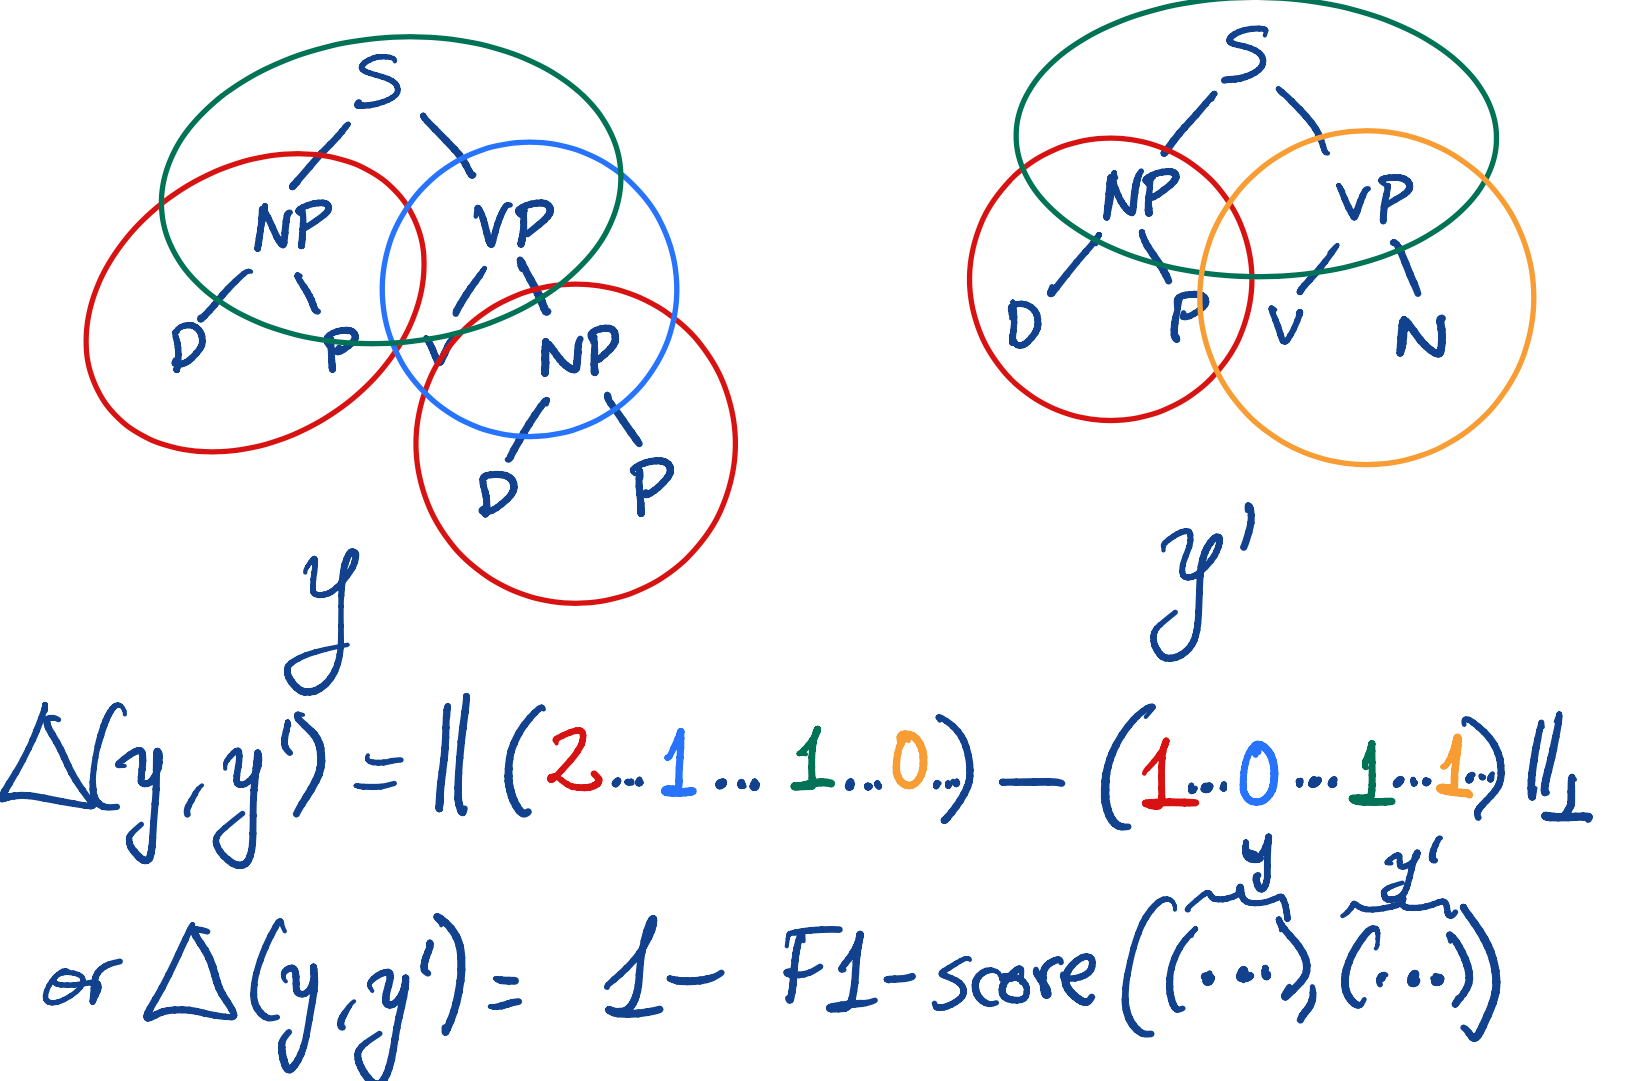
\includegraphics[width=.7\columnwidth]{images/8-ssvm-joint-feature-maps.png}
\end{center}

\textbf{Soft-margin Formulation}
\begin{equation*}
	\begin{gathered}
		\min_{w,\xi} \frac{1}{2} \norm{w}^2 + {\color{imp} \frac{C}{{\color{imp2}n}}\sumin \xi_i} \\
		\textit{s.t. }  w^T\Psi(x_i, y_i) \geq \Delta(y_i, y') + w^T\Psi(x_i, y') - {\color{imp} \xi_i} \\
		\xi_i \geq 0, \forall y'\neq y_i, i\leq n
	\end{gathered}
\end{equation*}
\textbf{Why the {\color{imp2}n}?}

Theorem: If $w^*. \xi^*$ are optimal, then the empirical risk of $w^*$ w.r.t $\Delta$ is 
\begin{align*}
	\E_{x,y}[\Delta (Y, c_w(x))] 	&= \frac{1}{n}\sumin\Delta(y_i, c_w(x_i)) \\
									&\leq \frac{1}{n} \sumin\xi_i
\end{align*} 
\textit{Proof on slide 42}

The conditions can also be written as: 
\begin{equation*}
	\begin{gathered}
		\textit{s.t. }  w^T\Psi(x_i, y_i) \geq 1 + + w^T\Psi(x_i, y') - \frac{{\color{imp} \xi_i}}{\Delta(y_i, y')} \\
		\xi_i \geq 0
	\end{gathered}
\end{equation*}
This formulation is \textbf{invariant to rescaling of $\mathbf \Delta$}




\subsubsection{Training Algorithm}
\begin{algorithm}[H]  
	\SetKwInOut{Input}{input}
	\Input{tolerance threshold $\epsilon > 0$}
	$\w\gets 0, \xi\gets 0, W\gets \emptyset$ \\
   \DoUntil{$W$ does not change}
   {
   		\For{$i\leq n$}
   		{
			$y'\gets \arg\max_{y\neq y_i} \left\{ \Delta(y_i, y) + w^T\Psi(x_i, y)\right\}$ 
			
			\If{$(w^T\Psi(x_i, y_i)$ $\not\geq$ $\Delta(y_i, y') + w^T(x_i, y') - \xi_i-\epsilon)$}{
				$ W\gets W \cup \left\{w^T\Psi(x_i, y_i) \geq \Delta(y_i, y') -\xi_i + w^T\Psi(x_i, y') \right\}$
			}      		
      	}
      	$w, \xi \gets \textit{solve}\left(\min_w \frac{1}{2} \norm{w}^2 + \frac{C}{n} \sum_i\xi_i \textit{ s.t. } W \right)$
  	}
  \caption{SVM training algorithm}
\end{algorithm}
	
\subsubsection{Prediction: }
$$
	c(x) = \arg\max_y w^T\Psi(x,y)
$$

\subsection{Advantages and Disadvantages}
\begin{center}
	\begin{tabular}{ p{0.45\columnwidth} | p{0.45\columnwidth} } 
		\textbf{Advantages} & \textbf{Disadvantages}\\\hline
			- Works well with infinitely dimensional representations & - requires careful model selection \\
			-  Adapted to structured classification & - Requires feature Engineering \\
			- Formulated as QP, for which efficient procedures are available & - Use of kernels make training algos succeptible to curse of dim
	
	\end{tabular}
\end{center}

\textit{Examples on page 51 - 64 (page ranking, diseases, ...)}
	
	
